%Introduction
The workings of the brain have intrigued researchers across various spectrums of science - from neuroscience to computer science. While the cortex still remains 
an enigma to the community, the visual cortex is a more finely understood system and many mathematical models mimicing the 
human visual system (HVS) have been proposed. Some of the early work in vision focused on understanding how primal capabilities of vision trigger higher modalities 
such as object recognition~\cite{marr}. Progressively, object recogntion models based on the simple and complex cells in the cortex were developed~\cite{Mutch2008}. 
To understand task-driven vision, attention models using salient features of 
a visual scene were proposed~\cite{Bruce2006, Itti2001}. More recent work focuses on understanding the impact of attention under the influence of multiple cues~\cite{wyble2014}.

%Motivate need for vision accelerators
Most of these vision models are computationally intensive that require frequent accesses to memory due to large matrix operations 
that run either in a feed-forward or an iterative manner. 
Running these workloads in real-time is a necessary constraint that needs 
to be met by the underlying system, but is becoming a daunting challenge with increasing resolutions of 
display panels coupled with improved camera sensors.

Given the challenges and opportunities in neuromorphic computing, many have embarked upon developing systems for smart vision applications. 
Synopys recently launced EV544 - a Convolutional Neural Network (CNN) based processor~\cite{syncnn}.
The SpiNNaker project has evolved from being a massively parallel representation of the human brain to now being used as a tool to further advance studies in 
neuroscience and robotics~\cite{spinnaker}. In a similar league, the True North chip~\cite{truenorth} meanders away from the traditional 
von Neumann architecture and uses 4096 parallel and distributed cores is an event-driven framework for solving problems in vision and audition.

\begin{figure}[!htb]
\vspace{0pt}
\centering
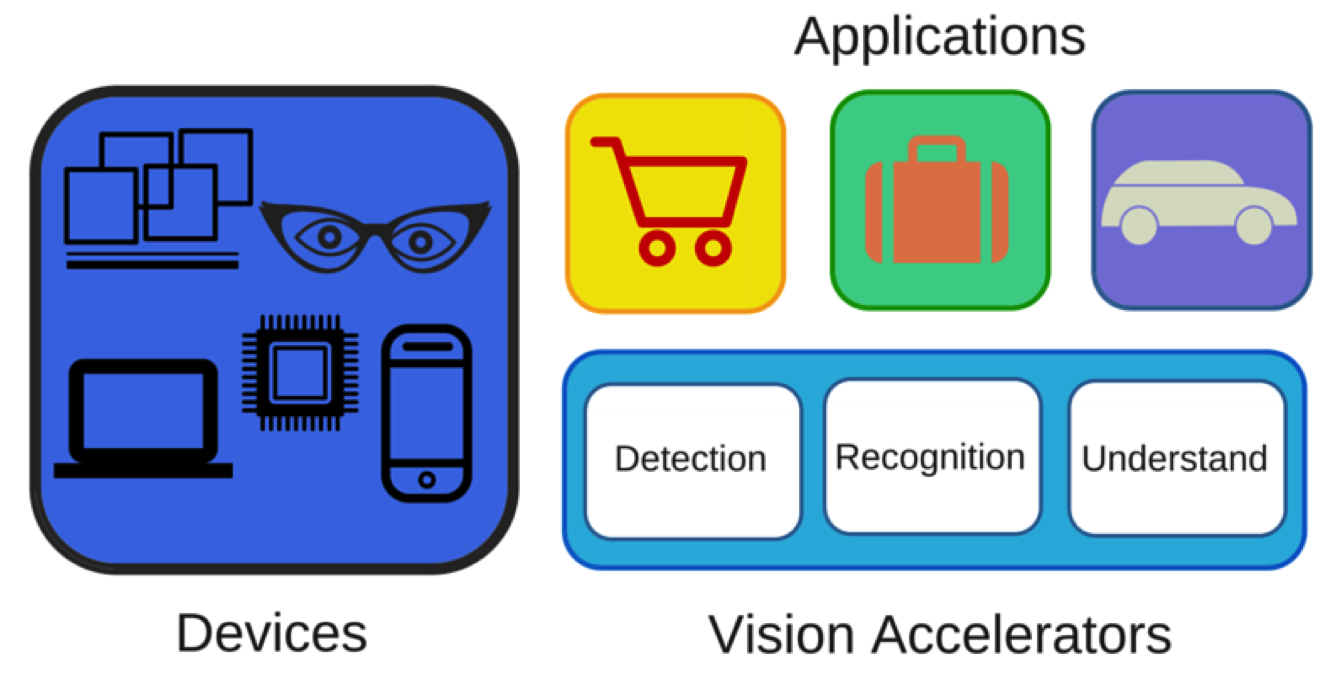
\includegraphics[width=0.9\linewidth]{./figures/vision_apps_devices.png}
\vspace{0pt}
\caption{Application-specific vision accelerator pipeline.}
\label{fig:iot}
\vspace{0pt}
\end{figure}

Fig.~\ref{fig:iot} illustrates the interaction between compute devices and vision accelerators when targeting various applications. A common vision pipeline involves parsing the visual scene and extracting objects or regions of interest (RoIs). This is 
carried out in the object detection stage. Once regions are extracted they are sent to a recognition stage to identify 
what the object is. Having figured out whether the object is of interest, further options can be explored. For example, if the 
object is a person, activity or pose estimation can be triggered. The application workload usually will decide the choice of 
the compute device. For example, if a user is in a retail store and would like to use a smart visual-assist device, a 
wearable small form-factor device would be ideal. However, if this is an automotive-assist system, a larger device may be 
engaged. If a security application is being deployed at an airport, then a large server-scale architecture would be needed to
handle the sheer volume of data being generated every minute.

The main contributions of this paper are:
\begin{itemize}
\item To usher in the next wave of technology, we explore the current state-of-the-art in 
embedded vision accelerators and lay emphasis on key insights when designing such accelerators.
\item With scaling technology paving the way for approximate computing, we exploit an increasingly powerful property of most vision algorithms - reliability to noise. 
We show that for an object recognition system using DRAMs for memory storage, we can reduce refresh rates by $4\times$ thus reducing refresh energy. We can also reduce the number of multipliers by $7\times$ in the preprocessing stage of the system. We maintain a 1\% error bound on accuracy while exploiting reliability of the system.
\end{itemize}

The rest of this paper is organized as follows:
In Section~\ref{sec:related}, we provide an overview of vision-based architectures and the corresponding state-of-the-art.
Section~\ref{sec:reliability} describes opportunities to optimize an object recognition application based on its error resilient capabilities.
Finally, we conclude with Section~\ref{sec:conclusion}.
